\section{Análisis de sensibilidad}
\label{sec:sensibilidad}

\subsection{Sensibilidades simbólicas}
Se usa la sensibilidad normalizada de un parámetro $P$ respecto de un componente $x$~\cite{daryanani1976,apuntes2026},
\begin{equation}
  S^P_x = \frac{x}{P}\frac{\partial P}{\partial x} = \frac{\partial \ln P}{\partial \ln x}
  \qquad\Longrightarrow\qquad \frac{\Delta P}{P} \approx S^P_x\,\frac{\Delta x}{x}.
  \label{eq:sens_def}
\end{equation}
Se calculó con SymPy sobre las expresiones generales de la \cref{eq:param_circuito}, \emph{antes} de imponer valores o relaciones entre componentes:
\begin{gather}
  S^{\omega_r}_{R_0} = -\frac{R_0}{R_0+R_s},\qquad S^{\omega_r}_{R_s} = -\frac{R_s}{R_0+R_s},\qquad S^{\omega_r}_{C_0} = -1, \label{eq:sens_wr}\\
  S^{\omega_0}_{R_1} = S^{\omega_0}_{R_2} = S^{\omega_0}_{C_1} = S^{\omega_0}_{C_2} = -\frac12, \label{eq:sens_w0}\\
  S^{Q}_{R_1} = -S^{Q}_{R_2} = \frac{R_2-R_1}{2(R_1+R_2)},\qquad S^{Q}_{C_1} = -S^{Q}_{C_2} = \frac12. \label{eq:sens_Q}
\end{gather}
La ganancia en continua es $H(0) = 1$ independientemente de los componentes, de modo que su sensibilidad es nula. No hay resistencias de ganancia del
AO porque ambos trabajan como seguidores. Se verifican además las propiedades de la cátedra: $\sum_R S^{\omega}_R = \sum_C S^{\omega}_C = -1$ para
$\omega_r$ y $\omega_0$ (homogeneidad de grado $-1$ en $R$ y en $C$), y $\sum_R S^Q_R = \sum_C S^Q_C = 0$, porque $Q$ es adimensional y no cambia con un
escaleo de impedancia ni de frecuencia.

La \cref{tab:sensibilidades} evalúa estas expresiones con los componentes adoptados. Para una resistencia formada por dos en serie,
$R = R_a + R_b$, la regla de la cadena da $S^P_{R_a} = S^P_R\,R_a/R$: las resistencias de ajuste (\qty{560}{\ohm}, \qty{3.3}{\kilo\ohm}) aportan
poco, y la tolerancia de \qty{1}{\percent} de cada una se pondera por su fracción del total.

\begin{table}[H]
  \centering\small
  \caption{Sensibilidades normalizadas evaluadas en los componentes adoptados. Abajo, las resistencias individuales de cada par en serie.}
  \label{tab:sensibilidades}
  \tabres{tab_sensibilidades}
\end{table}

Lectura de la tabla:
\begin{itemize}
  \item $\omega_r$ depende prácticamente solo de $R_0$ y $C_0$ ($S \approx -1$). El generador aporta $S^{\omega_r}_{R_s} = \num{-0.0024}$.
  \item $\omega_0$ tiene sensibilidad $-\tfrac12$ respecto de los cuatro elementos del Sallen--Key, cualquiera sea el diseño.
  \item $Q$ depende de los capacitores con $\pm\tfrac12$ y de las resistencias con apenas $\pm\num{0.095}$, gracias a que $R_1 \approx R_2$
        (\cref{sec:sintesis}). \textbf{Los componentes críticos son los capacitores}, que además son los de mayor tolerancia.
\end{itemize}

\subsection{Validación por perturbaciones finitas}
Para validar las expresiones en forma independiente, cada componente se perturbó en $\pm\qty{1}{\percent}$. En cada caso se recalcularon $\omega_r$,
$\omega_0$ y $Q$ a partir de las \emph{raíces del denominador} de $H_c(s)$, evaluado numéricamente, y no de las fórmulas cerradas. Se estimó la
sensibilidad con diferencias unilaterales y con la diferencia central logarítmica
$S \approx [\ln P(x(1+\delta)) - \ln P(x(1-\delta))]/[\ln(1+\delta)-\ln(1-\delta)]$, con $\delta = 0{,}01$ (\cref{tab:validacion_sens}).

\begin{table}[H]
  \centering\small
  \caption{Sensibilidades simbólicas frente a perturbaciones de $\pm\qty{1}{\percent}$ (solo las no nulas).}
  \label{tab:validacion_sens}
  \tabres{tab_validacion_sens}
\end{table}

Las diferencias unilaterales se apartan de la sensibilidad simbólica en el término de segundo orden ($\approx \tfrac12\,\delta\,S(S-1)$ para
$P \propto x^S$, es decir, $\approx \num{0.01}$ para $S = -1$). La diferencia central lo cancela y coincide con la simbólica con un error menor que
\num{\vMaxErrCentral}. Con $\pm\qty{1}{\percent}$ la aproximación lineal es excelente: el cambio porcentual real difiere del predicho en centésimas de
punto porcentual.

\subsection{Efecto del amplificador operacional}
Con $A(s) = \omega_t/s$ en ambos AO y GBW de \qty{3}{\mega\hertz}, el GBW finito desplaza $f_0$ en \qty{\vDfoGBW}{\percent} y $Q$ en
\qty{\vDQGBW}{\percent}, mientras que $\omega_r$ no se modifica. La sensibilidad de $Q$ respecto del GBW es $S^Q_{\mathrm{GBW}} = \num{\vSQGBW}$: una
variación de \qty{50}{\percent} del GBW entre unidades o revisiones del TL072 cambiaría $Q$ en menos de \qty{0.04}{\percent}. El AO no es un
elemento crítico de este diseño.

\subsection{Sensibilidad de la magnitud y dispersión esperada}
La parte real de la sensibilidad de la función, $S^{|H|}_x(\omega) = \mathrm{Re}\{(x/H)\,\partial H/\partial x\}$, indica cuánto cambia la magnitud
en cada frecuencia (\cref{fig:sens_magnitud}). En la banda de paso baja todas son prácticamente nulas, porque $H(0) = 1$ por construcción. Cerca del
borde, en \qty{1}{\kilo\hertz}, dominan $R_0$ y $C_0$ ($\approx \num{-0.62}$) y $C_1$ ($\num{\vSHmilCuno}$). En la banda de rechazo todas tienden a
$-1$, que es la sensibilidad de un pasabajos de orden~3 por encima de sus polos: la atenuación crece \qty{0.087}{\decibel} por cada
\qty{1}{\percent} de aumento de cualquier $R$ o $C$.

\begin{figure}[H]
  \centering
  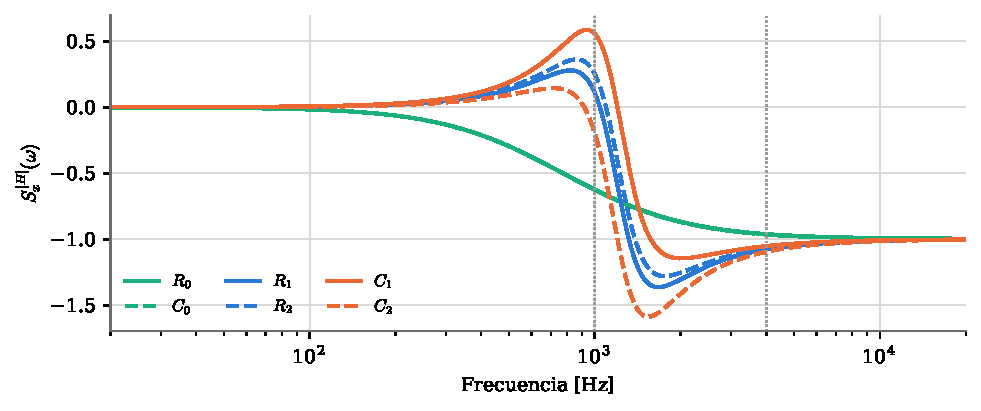
\includegraphics[width=0.9\linewidth]{fig_sens_magnitud}
  \caption{Sensibilidad de la magnitud respecto de cada componente. Las líneas punteadas son los bordes de la plantilla (\qty{1}{\kilo\hertz} y
  \qty{4}{\kilo\hertz}).}
  \label{fig:sens_magnitud}
\end{figure}

Con variaciones independientes y uniformes de semiancho $t_x$ ($\sigma_x/x = t_x/\sqrt3$), la desviación estándar de la magnitud en dB es
\begin{equation}
  \sigma_{|H|,\mathrm{dB}}(\omega) \approx \frac{20}{\ln 10}\sqrt{\sum_x \left(S^{|H|}_x(\omega)\right)^2 \left(\frac{t_x}{\sqrt3}\right)^2}.
\end{equation}
En la banda de paso, el máximo está en el borde de \qty{1}{\kilo\hertz}: \qty{\vSigCincoPaso}{\decibel} con capacitores de
$\pm\qty{5}{\percent}$ y \qty{\vSigDiezPaso}{\decibel} con $\pm\qty{10}{\percent}$ (\cref{fig:banda_dispersion}). Con $\pm 2\sigma$ la banda queda
dentro de la plantilla para capacitores de $\pm\qty{5}{\percent}$ y apenas la toca para $\pm\qty{10}{\percent}$, en coincidencia con el
rendimiento estimado en la \cref{sec:margen}. A \qty{4}{\kilo\hertz}, la dispersión ($\sigma \le \qty{\vSigDiezCuatro}{\decibel}$) es despreciable
frente a los \qty{10.7}{\decibel} de margen.

\begin{figure}[H]
  \centering
  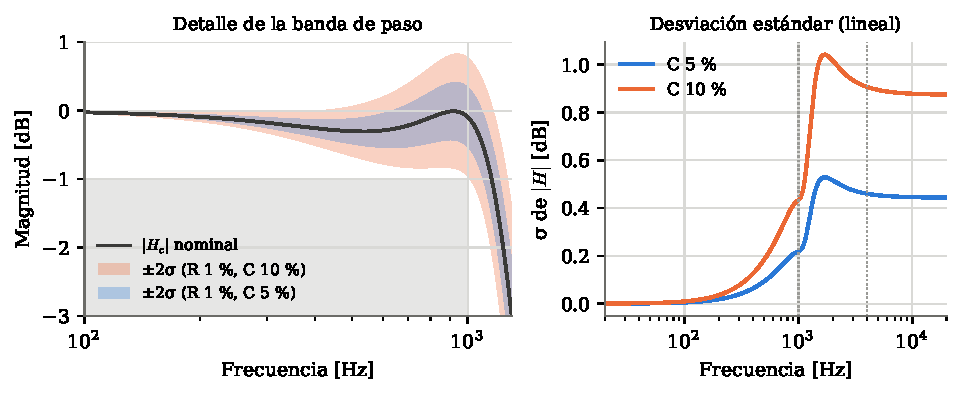
\includegraphics[width=\linewidth]{fig_banda_dispersion}
  \caption{Izquierda: magnitud nominal y banda $\pm 2\sigma$ en la banda de paso (zona gris: región prohibida). Derecha: desviación estándar de
  $|H|$ en función de la frecuencia.}
  \label{fig:banda_dispersion}
\end{figure}

\subsection{Predicción lineal de la dispersión de los parámetros}
La predicción de primer orden para variables independientes, $(\sigma_P/P)^2 \approx \sum_x (S^P_x)^2(\sigma_x/x)^2$, se contrastó con un Monte
Carlo de \num{100000} muestras sobre las expresiones exactas (\cref{tab:dispersion_lineal}). La coincidencia es muy buena: la desviación estándar
lineal difiere de la muestral en menos de \qty{1}{\percent} relativo. El sesgo de la media es pequeño y crece con la tolerancia (es un efecto de
segundo orden: $\omega \propto x^{-1}$ o $x^{-1/2}$ es convexa). El contraste con el Monte Carlo de LTspice forma parte del Nivel~II.

\begin{table}[H]
  \centering\small
  \caption{Dispersión relativa de $\omega_r$, $\omega_0$ y $Q$: predicción lineal frente a Monte Carlo ($R$: $\pm\qty{1}{\percent}$, uniforme).}
  \label{tab:dispersion_lineal}
  \tabres{tab_dispersion_lineal}
\end{table}
